\section{Introduction} \label{section:introduction}

% Common LLM-based agentic systems
Large language models\,(LLMs) have catalyzed the development of agentic systems capable of executing complex, multi-step tasks autonomously\,\citep{MetaGPT_ICLR_24, AutoGen_COLM_24, AgentGym_24, GAIA_ICLR_24}. These systems, often constructed through meticulous manual engineering, integrate components such as Chain-of-Thought reasoning, tool invocation, and memory management to enable sophisticated behaviors for orchestrating intricate workflows\,\citep{rise_agent_survey_25, LLMReasoning_Survey_25, AgenticAI_Survey_25, ALLM_Survey_25}. However, the handcrafted nature of these systems imposes limitations on scalability, adaptability, and rapid deployment across diverse domains.


% From manual to automated design of agentic systems
To address these limitations, recent trends have shifted towards automated design methods for agentic systems\,\citep{ADAS_ICLR_25, AgentSquare_ICLR_25, AFlow_ICLR_25, GPTSwarm_ICML24, DyLAN_COLM_24, EvoMAC_ICLR_25, EvoAgent_NAACL_25}. Automated methods typically employ search algorithms to discover optimal workflow configurations by systematically exploring a vast design space. Instead of relying on human intuition, these approaches generally involve iterations of candidate generation, evaluation, and refinement. While promising, these methods exhibit significant drawbacks, chiefly the high computational costs associated with the extensive validation steps needed during the exploration and evaluation phases of the search. Each candidate configuration must undergo rigorous evaluation, often through expensive, repeated interactions with LLM APIs, rendering the search prohibitively costly and time-consuming.


% Limitations of automated design --> Prediction-based search
In this paper, we argue that purely search-based automated design methods are inherently inefficient and propose a predictive approach to significantly accelerate workflow evaluation. Specifically, we advocate for a predictor-based framework that can rapidly estimate the performance of candidate agentic workflows, similar to performance predictors in neural architecture search\,\citep{powerful_nas_predictor_NeurIPS_21}, thereby reducing the need for extensive validation. 

\begin{wrapfigure}{r}{0.5\textwidth}
    % \vspace*{-0.5cm}
    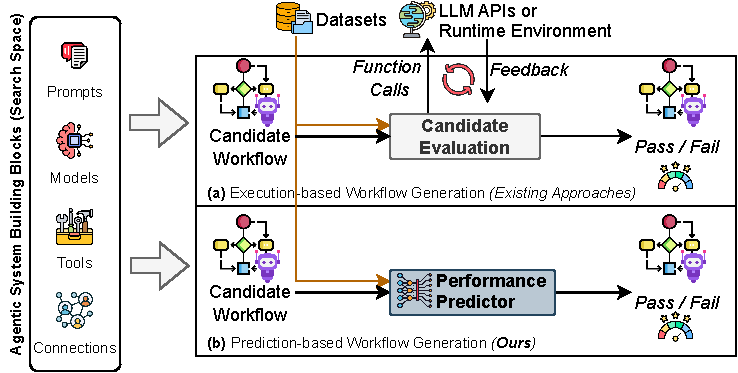
\includegraphics[width=0.5\textwidth]{figures/comparison.pdf}
    \vspace*{-0.5cm}    
    \caption{Comparison between (a) execution-based and (b) prediction-based candidate evaluation for agentic workflow generation. Execution-based methods rely on costly runtime or LLM calls, while our prediction-based approach offers faster, scalable evaluation via a learned predictor.} \label{figure:comparison}
    \vspace*{-0.5cm}
\end{wrapfigure}

As depicted in \autoref{figure:comparison}, instead of fully evaluating every candidate, a predictive model can estimate the quality and viability of agentic workflows, thus guiding the search process far more efficiently. By reducing costly ground-truth executions or environment interactions during the search process, prediction-based approaches promise significant improvements in both search efficiency and solution quality. However, building a high-quality predictor for agentic workflows introduces two fundamental challenges.


% Challenges of prediction-based search
\textbf{Workflow Heterogeneity}. Agentic workflows exhibit considerable heterogeneity; subtle variations in configuration can lead to dramatically different performances. Specifically, workflows can vary widely in communication structure, prompting strategies, tool invocation patterns, and reasoning styles, making it challenging to learn a unified predictive model. Moreover, agentic systems differ significantly across tasks, domains, and toolsets, resulting in diverse and complex workflow configurations that are difficult to model uniformly\,\citep{TheAgentCompany_24, WorFBench_ICLR_25}.

\textbf{Scarcity of Labeled Data}. The availability of labeled data for training effective prediction models is severely limited due to the prohibitive cost of generating performance labels through exhaustive validation. Constructing a large, diverse set of labeled workflows with known execution outcomes is particularly expensive, creating a data bottleneck for supervised learning approaches. Moreover, gathering large-scale, high-quality labels for agentic workflows (e.g., success rates and execution outcomes) is often infeasible, further limiting the amount of supervised training data available for learning accurate predictors.


% Our main idea + Figure 1
% Extra points for having Figure 1 on the first page
% % 2: New trend: specifically list your contributions as bullet points (credits to Brendan)

To tackle these challenges, we present \textbf{\ours{}}, a multi-view encoder framework for performance prediction in LLM-based agentic workflows. To address workflow heterogeneity, \ours{} uses \emph{multi-view workflow encoders} that jointly model complementary signals---structural\,(e.g., agent topology), behavioral\,(e.g., tool usage), and semantic (e.g., prompts)---capturing the diverse, task-dependent characteristics of workflow configurations. To mitigate label scarcity, we introduce \emph{cross-domain unsupervised pretraining}, denoted \ours{}+, which leverages abundant unlabeled workflows from related domains. We pretrain the multi-view encoders with contrastive and reconstruction objectives, then fine-tune on limited labeled data, yielding robust and transferable representations for prediction. The \textbf{main contributions} of this paper are as follows.

\begin{itemize}[leftmargin=10pt, nosep, noitemsep]
    \item We propose multi-view encoders and cross-domain unsupervised pretraining that jointly capture the heterogeneous facets of LLM-based agentic workflows, yielding higher predictive performance, better generalization, and effective predictor training under limited labels.    
    
    \item We introduce \ours{}, unifying these components for the underexplored problem of performance prediction in heterogeneous, label-scarce LLM-based agentic workflows, thereby reducing trial-and-error costs and accelerating development.
    
    \item We empirically demonstrate that, averaged across three domains, \ours{} improves prediction accuracy by up to \textbf{6.90\%} and utility by up to \textbf{5.87\%} over strong baselines.
\end{itemize}



